% IEEE standard conference template; to be used with:
%   spconf.sty  - LaTeX style file, and
%   IEEEbib.bst - IEEE bibliography style file.
% --------------------------------------------------------------------------

\documentclass[letterpaper]{article}
\usepackage{spconf,amsmath,amssymb,graphicx}
\usepackage[utf8]{inputenc} 			% Zeichensatz
\usepackage[T1]{fontenc} 			% Umlaute unterstützen
\usepackage{float}

% Example definitions.
% --------------------
% nice symbols for real and complex numbers
\newcommand{\R}[0]{\mathbb{R}}
\newcommand{\C}[0]{\mathbb{C}}

% bold paragraph titles
\newcommand{\mypar}[1]{{\bf #1.}}

% Title.
% ------
\title{Parallel implementation of Fringe Search}
%
% Single address.
% ---------------
\name{Lukas Mosimann, Christian Zeman} 
\address{ETH Z\"urich\\Z\"urich, Switzerland}

% For example:
% ------------
%\address{School\\
%		 Department\\
%		 Address}
%
% Two addresses (uncomment and modify for two-address case).
% ----------------------------------------------------------
%\twoauthors
%  {A. Author-one, B. Author-two\sthanks{Thanks to XYZ agency for funding.}}
%		 {School A-B\\
%		 Department A-B\\
%		 Address A-B}
%  {C. Author-three, D. Author-four\sthanks{The fourth author performed the work
%		 while at ...}}
%		 {School C-D\\
%		 Department C-D\\
%		 Address C-D}
%

\begin{document}
%\ninept
%
\maketitle
%

\begin{abstract}
Describe in concise words what you do, why you do it (not necessarily
in this order), and the main result.  The abstract has to be
self-contained and readable for a person in the general area. You
should write the abstract last.
\end{abstract}

\section{Introduction}\label{sec:intro}

This project was part of the course \textit{Design of Parallel and High-Performance Computing} given by Torsten Hoefler and Markus Püschel in autumn 2013 at ETH Zürich.


\mypar{Motivation} 
Pathfinding is an important part in many applications, especially in computer games and robotics. Fringe search is a popular algorithm for single-pair shortest path problems. Unlike A* it won't guarantee to find the shortest path, but rather a path "short enough". The advantage of Fringe Search is that it generally outperforms A* as shown in \cite{fringe:05}.\\
In \cite{brand:09} a parallel implementation of Fringe Search has been done for a distributed memory environment. The goal of this paper was the implementation and benchmarking of a parallel version of Fringe Search for a shared memory environment.

\mypar{Related work} This paper is mainly based on two papers. The Fringe Search algorithm was introduced in \cite{fringe:05}. S. Brand and R. Bidarra implemented a parallel version in a distributed memory environment described in \cite{brand:12} and a bit more specific in the Master Thesis of S. Brand \cite{brand:09}. In this paper the implementation was done for a shared memory environment.

\section{Background: Shortest Path Problem}\label{sec:background}
In this section we formally define the single-pair shortest path problem we consider and introduce two algorithms that are used to solve it.

\mypar{Single-pair shortest path problem}
A problem where the goal is to find the shortest path between a start and an end node in a directed or undirected graph. In our case we used a directed graph.

\mypar{A*}
A very popular algorithm that uses a best-first search approach for solving the single-pair shortest path problem. For the best-first search it uses a heuristic function (e.g. Euclidean distance to end node). It always finds the shortest possible path and therefore it's called optimal. It uses a priority queue for the nodes and therefore each insert into the queue has complexity $O(\log n)$.

\mypar{Fringe Search}
A single-pair shortest path algorithm that is similar to A*, but instead of a priority queue that always has the most promising node first, it stores the nodes in a simple list where an insert has the complexity $O(1)$ and visits a node if it's "promising enough" which is determined by a global threshold value that will be continuously increased. It's not optimal (it doesn't guarantee to find the shortest path) but it is generally faster than A*, as shown in \cite{fringe:05}. An example of the algorithm can be found in figure \ref{fringe:algo}.

\begin{figure}[h]\centering
  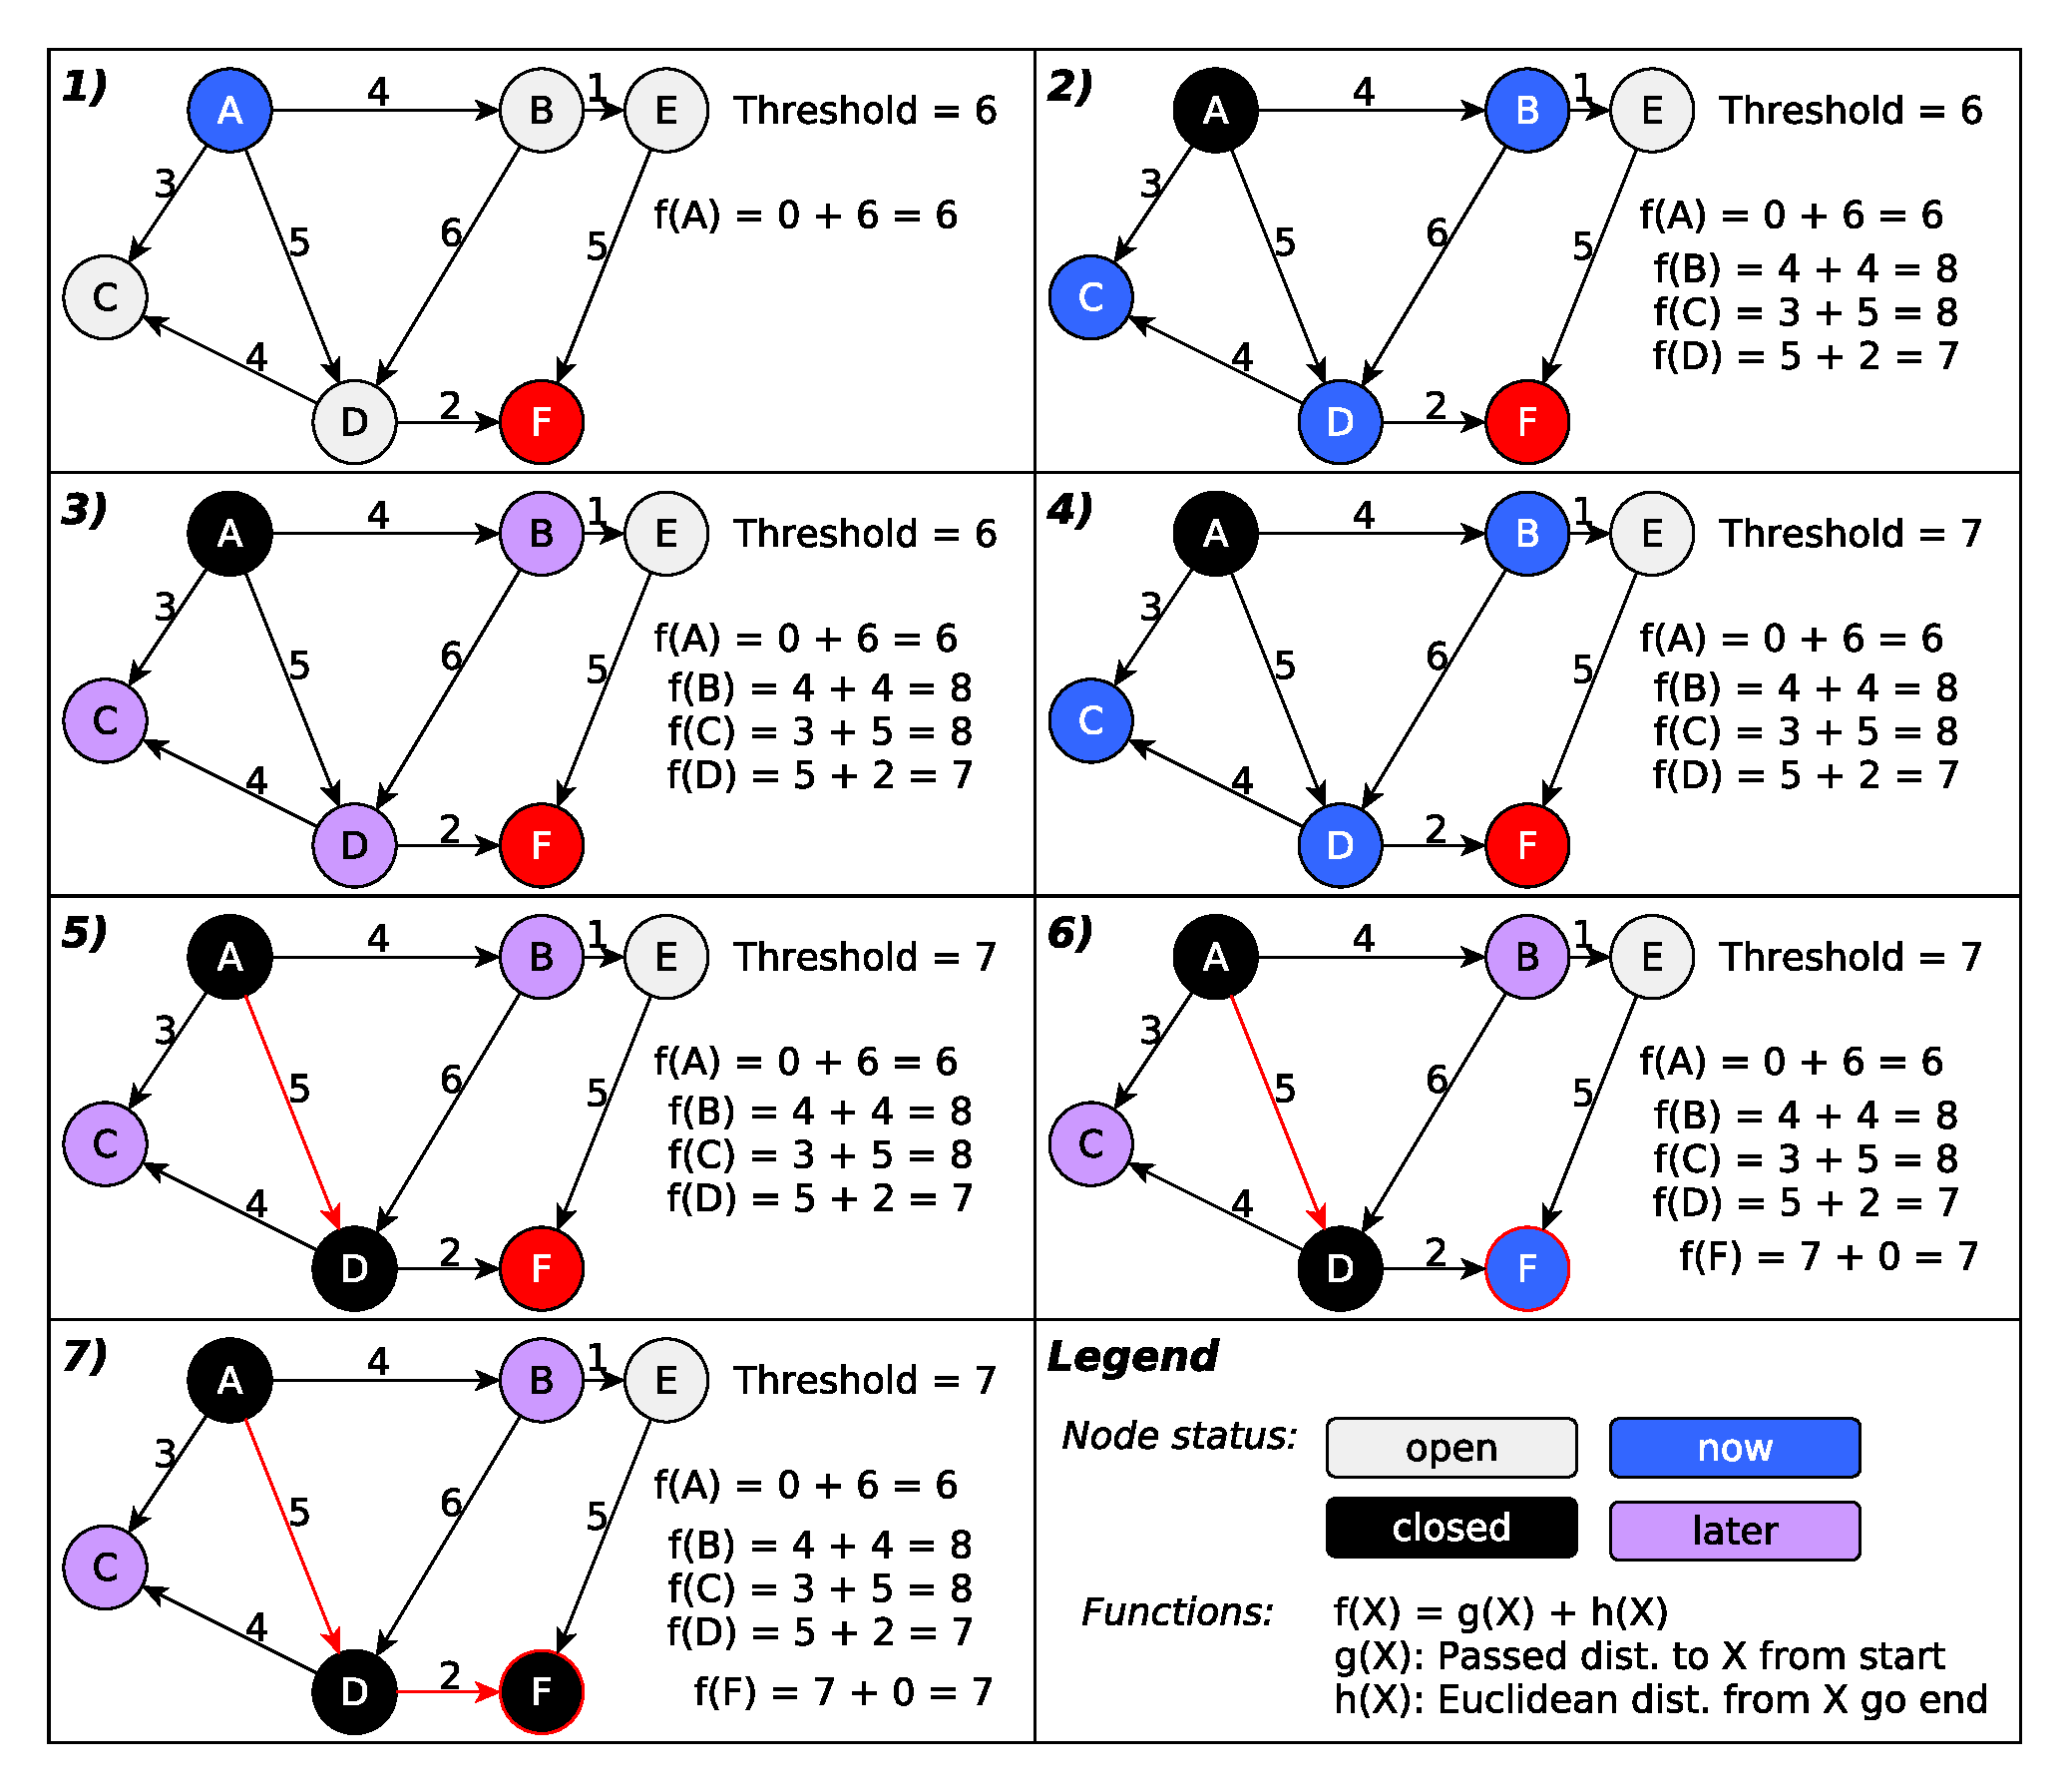
\includegraphics[scale=0.245]{fringe_rep.eps}
  \caption{Fringe Search example \label{fringe:algo}}
\end{figure}


\section{Your Proposed Method}\label{sec:your method}

Now comes the ``beef'' of the report, where you explain what you
did. Again, organize it in paragraphs with titles. As in every section
you start with a very brief overview of the section.

In this section, structure is very important so one can follow the technical content.

Mention and cite any external resources that you used including libraries or other code.

\section{Experimental Results}\label{sec:exp}

Here you evaluate your work using experiments. You start again with a
very short summary of the section. The typical structure follows.

\mypar{Experimental setup} Specify the platform (processor, frequency, maybe OS, maybe cache sizes)
as well as the compiler, version, and flags used. If your work is about performance, 
I strongly recommend that you play with optimization flags and consider also icc for additional potential speedup.

Then explain what kind of benchmarks you ran. The idea is to give enough information so the experiments are reproducible by somebody else on his or her code.
For sorting you would talk about the input sizes. For a tool that performs NUMA optimization, you would specify the programs you ran.

\mypar{Results}
Next divide the experiments into classes, one paragraph for each. In each class of experiments you typically pursue one questions that then is answered by a suitable plot or plots. For example, first you may want to investigate the performance behaviour with changing input size, then how your code compares to external benchmarks.

For some tips on benchmarking including how to create a decent viewgraph see pages 22--27 in \cite{Pueschel:10}.

{\bf Comments:}
\begin{itemize}
\item Create very readable, attractive plots (do 1 column, not 2 column plots
for this report) with readable font size. However, the font size should also not be too large; typically it is smaller than the text font size.
An example is in Fig.~\ref{fftperf} (of course you can have a different style).
\item Every plot answers a question. You state this question and extract the
answer from the plot in its discussion.
\item Every plot should be referenced and discussed.
\end{itemize}

%\begin{figure}\centering
%  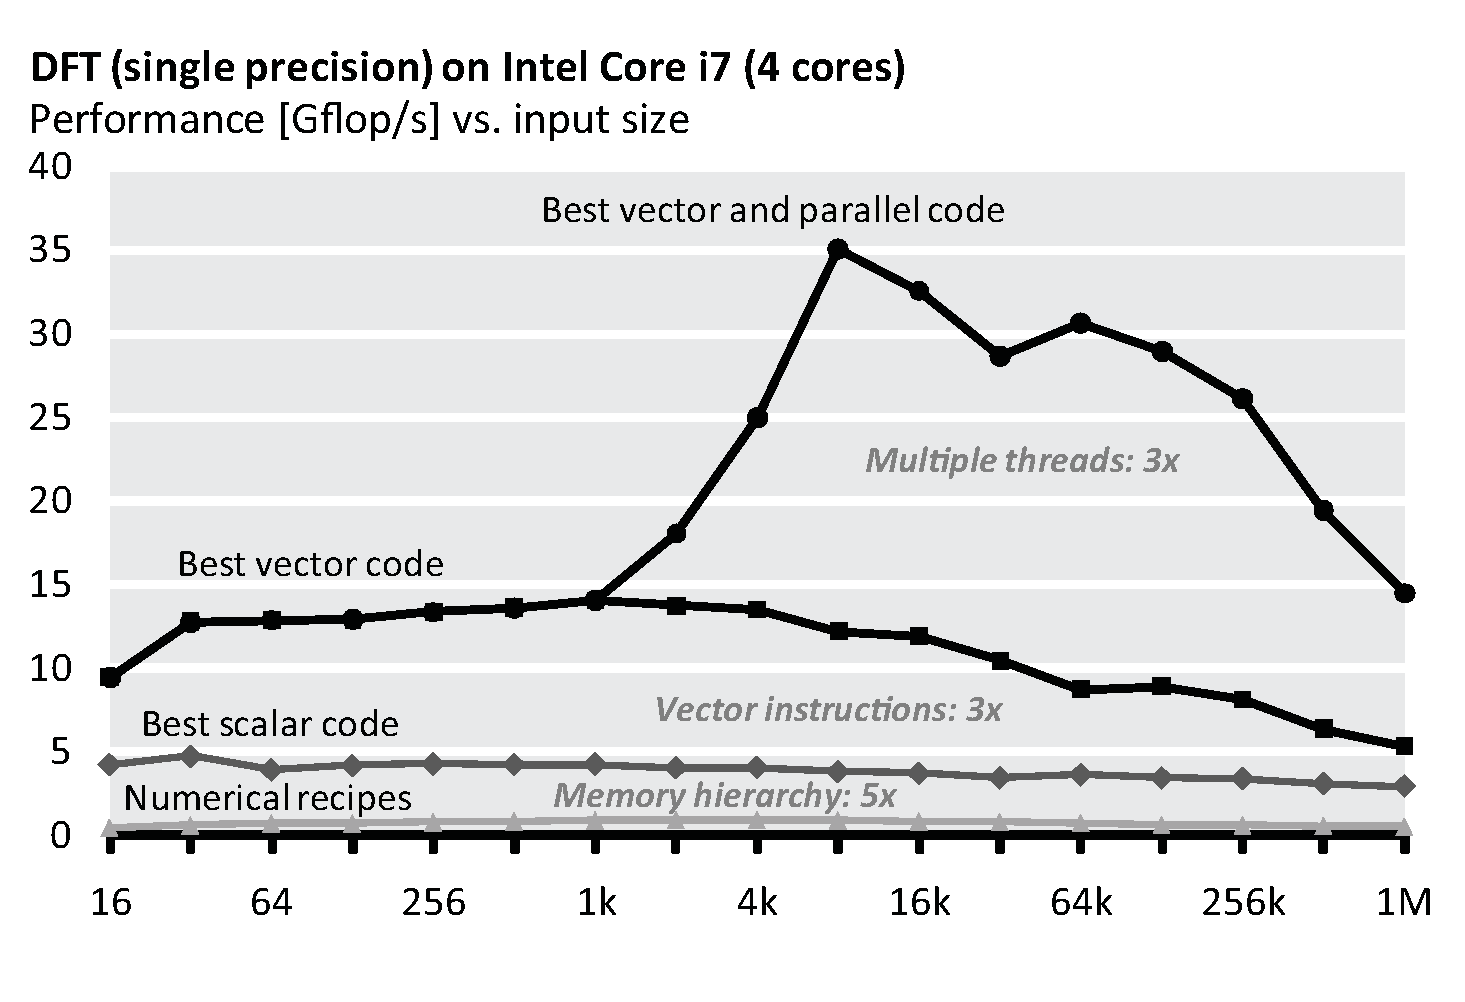
\includegraphics[scale=0.33]{dft-performance.eps}
%  \caption{Performance of four single precision implementations of the
%  discrete Fourier transform. The operations count is roughly the
%  same. The labels in this plot are maybe a little bit too small.\label{fftperf}}
%\end{figure}

\section{Conclusions}

Here you need to summarize what you did and why this is
important. {\em Do not take the abstract} and put it in the past
tense. Remember, now the reader has (hopefully) read the report, so it
is a very different situation from the abstract. Try to highlight
important results and say the things you really want to get across
such as high-level statements (e.g., we believe that .... is the right
approach to .... Even though we only considered x, the
.... technique should be applicable ....) You can also formulate next
steps if you want. Be brief. After the conclusions there are only the references.

\section{Further comments}

Here we provide some further tips.

\mypar{Further general guidelines}

\begin{itemize}
\item For short papers, to save space, I use paragraph titles instead of
subsections, as shown in the introduction.

\item It is generally a good idea to break sections into such smaller
units for readability and since it helps you to (visually) structure the story.

\item The above section titles should be adapted to more precisely
reflect what you do.

\item Each section should be started with a very
short summary of what the reader can expect in this section. Nothing
more awkward as when the story starts and one does not know what the
direction is or the goal.

\item Make sure you define every acronym you use, no matter how
convinced you are the reader knows it.

\item Always spell-check before you submit (to us in this case).

\item Be picky. When writing a paper you should always strive for very
high quality. Many people may read it and the quality makes a big difference.
In this class, the quality is part of the grade.

\item Books helping you to write better: \cite{Higham:98} and \cite{Strunk:00}.

\item Conversion to pdf (latex users only): 

dvips -o conference.ps -t letter -Ppdf -G0 conference.dvi

and then

ps2pdf conference.ps
\end{itemize}

\mypar{Graphics} For plots that are not images {\em never} generate the bitmap formats
jpeg, gif, bmp, tif. Use eps, which means encapsulate postscript. It is
scalable since it is a vector graphic description of your graph. E.g.,
from Matlab, you can export to eps.

The format pdf is also fine for plots (you need pdflatex then), but only if the plot was never before in the format 
jpeg, gif, bmp, tif.


% References should be produced using the bibtex program from suitable
% BiBTeX files (here: bibl_conf). The IEEEbib.bst bibliography
% style file from IEEE produces unsorted bibliography list.
% -------------------------------------------------------------------------
\bibliographystyle{IEEEbib}
\bibliography{bibl_conf}

\end{document}

